\chapter{SHMPO (SHared Annotator for Multiple Problems) Algorithms}

I this chapter, we describe algorithms for multi-task learning with
a shared annotator setting, that uses linear models. We start with a basic first order SHAMPO algorithm 
which is based on the perceptron algorithm 
and continue to number of algorithms that extends the basic one. Two steps are
yet to be specified: how to pick a task to be labeled at each round and how to
perform an update, once the true label for that task is given.. 

\section{SHAMPO perceptron}

We focus here on linear-functions of the form $f(\vx)=\sign(p)$ for the
quantity $p=\vwt\vx$, $\vw\in\reals^d$,  which often called the
\textit{margin}.
Specifically, the algorithm maintains a set of $K$ weight
vectors, $\vwi{i,t},~i\in\braces{1\comdots K}$. On round $t$, the algorithm predicts a label for each
 one of the tasks, $\hyi{i,t}=\sign(\hat{p}_{i,t})$ where $\hat{p}_{i,t}=\vwti{i,t-1}\vxiit$. 
 On rounds for which the label of some task $J_t$ is queried, the algorithm update the model of the
 queried task only, such that for the rest of the tasks, $i\neq J_t$, we have $\vwi{i,t}=\vwi{i,t-1}$ and no
 update is made for those unqueried tasks.       

We say that the algorithm has a prediction mistake on task $i$ in round $t$ if
$\yi{i,t} \neq \hyi{i,t}$, and denote this event by the indicator $M_{i,t}=1$,
otherwise, if there is no mistake, we set $M_{i,t}=0$. The goal of the
algorithm is to minimize the cumulative mistakes, $\sum_t \sum_i
M_{i,t}$. Models are also evaluated using the
{\em Hinge-loss}. Specifically, let $\vui{i}\in\reals^d$ be some vector
associated with problem $i$. We denote the Hinge-loss of it, with respect
to some input-label  pair $\paren{\vxiit,\yiit}$, by
$\lossp{\gamma,i,t}(\vui{i})= \paren{\gamma-\yiit
  \vuti{i}\vxiit}_+$, where, $(x)_+=\max\{x,0\}$, and $\gamma>0$ is
some parameter. The cumulative loss over all tasks and a sequence of
$n$ input steps, is
$ L_{\gamma,n} =L_{\gamma}(\{ \vui{i} \})=\sum_{t=1}^{n} \sum_{i=1}^{K}\ {\lossp{\gamma,i,t}(\vui{i})}$.
We also use the following expected hinge-loss over the random queried choices
of the algorithm, 
\begin{equation}
\bar{L}_{\gamma,n}=\bar{L}_{ \{ \vui{i}\}}
=\Exp{\sum_{t=1}^n \sum_{i=1}^{K}{M_{i,t}Z_{i,t}\lossp{\gamma,i,t}(\vui{i})}}. 
 \end{equation}
Now, we proceed by  describing our algorithm and specify how to choose a task to query its label,
 and how to perform an update.
 

In order to select a task to query on, the algorithm uses the absolute value of the margin 
$\hat{p}_{i,t}$. We can see $\abs{\hat{p}_{i,t}}$ as the certainty measure of the label prediction.
 intuitively if $\abs{\hat{p}_{i,t}}$ is small,
then there is uncertainty about the labeling of $\vxi{i,t}$, and vice-versa for 
large values of $\abs{\hat{p}_{i,t}}$. 
Similar argument was used by ~\cite{DBLP:conf/icml/TongK00} for picking an example to be labeled in 
batch active learning. 
Example for the using of the margin as a certainty measure is shown in \figref{fig:margin} which illustrated 
a state of a linear binary classification algorithm of two dimensional problem. 
The circles and crosses represent two different classes and the separate hyperplane is shown. 
One of the circles examples have lower margin than the other, so its label can easily been replaced 
with the other one.
Prima facie, under this claim, at each point we should query the true label for the task
 that corresponds to the smallest margin.  Yet, if the model $\vwi{i,t-1}$ is not accurate enough, due to
 small number of observed examples, this estimation may be rough, and may lead to a wrong
conclusion. We thus perform an exploration-exploitation strategy, and
query tasks randomly, with a bias towards tasks with low margin
$\vert \hat{p}_{i,t} \vert$. 

\begin{figure}[h]
\begin{centering}
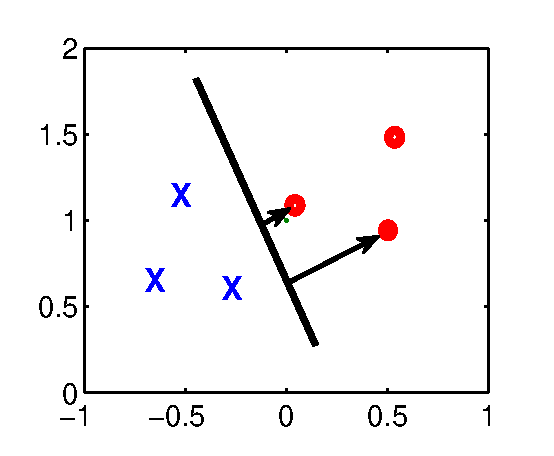
\includegraphics[width=0.5\textwidth]{figs/margin.eps}
\caption{Example for the using of the margin as a certainty measure.}
\label{fig:margin}
\end{centering}
\end{figure}


To the best of our knowledge,
exploration-exploitation usage in this context of choosing an examples
to be labeled (e.g. in settings such as semi-supervised learning or
selective sampling) is novel and new.  In order to get this property, we induced a
distribution over the tasks in the time step $t$, such that the probability to issue a query on the task 
$j$ ( $j=1 \comdots K$) is:

\begin{equation}
\begin{aligned}
\pr{J_t=j}&=\frac{\paren{b+\abs{\hat{p}_{j,t}}-\min_{m=1}^K\abs{\hat{p}_{m,t}}}^{-1}}{D_t}\\
~ \textrm { for } ~
D_{t}&=\sum_{i=1}^{K}{\paren{b+\abs{\hat{p}_{i,t}}-\min_{m}\abs{\hat{p}_{m,t}}}^{-1}}.
\label{eq:prob}
\end{aligned}
\end{equation} 
%
where $m=1 \comdots K$ and $b\geq 0, b\in\reals$ is a tradeoff parameter, between exploration and
exploitation. Clearly, it is a distribution, since $\pr{J_t=j}\geq 0$ and $\sum_j \pr{J_t=j}=1$. 
When we examine the extreme cases  of $b$ we see that  for $b\rightarrow0$
we have $\pr{J_t=j}\rightarrow1$ for the task with minimal margin, $J_t=\arg\min_{i=1}^K\abs{\hat{p}_{i,t}}$,  and $\pr{J_t=j}\rightarrow0$ for all the rest. In this case , pure exploitation is being made. The pure exploration happens when   $b\rightarrow \infty$
, then the distribution is uniform, $ \pr{J_t=j}= 1/K,~~ \forall j $. \figref{fig:probability_example} 
shows an example of this distribution for the case of two tasks ($K=2$) at an arbitrary step $t^*$. 
For visualization purpose, we fix 
$\abs{\hat{p}_{2,t^*}}=0.5$ and see how the probability of task $1$ to be chosen,
 is affected by varying $b$ and $\abs{\hat{p}_{1,t^*}}$ values. 
 Three different vertical areas  can be easily seen 
in the graph. The upper (green) area, where $b>>\max{\braces{\abs{\hat{p}_{1,{t^*}}},\abs{\hat{p}_{2,t{^*}}}}$,
 shows uniform distribution ($\pr{J_{t^*}=2}=\pr{J_{t^*}=1}=1/K=0.5$) 
 which represents the exploration over the tasks.
 In the lower area, the probability is compatible with the exploitation method and is changing between
 probability $1$ in the left, and probability $0$ to the right with a sharp threshold at $\abs{\hat{p}_{1,t^*}}=0.5$, 
 which is very close to the delta distribution $\pr{J_{t^*}=1}=\mathbb{I}\brackets{\hat{p}_{1,{}t^*}<\hat{p}_{2,{t^*}}}$.
 Whereas, the intermediate area, is the exploration-exploitation area that is 
 given by a distribution that is biased toward the lowest margin task.

\begin{figure}[h]
\begin{center}
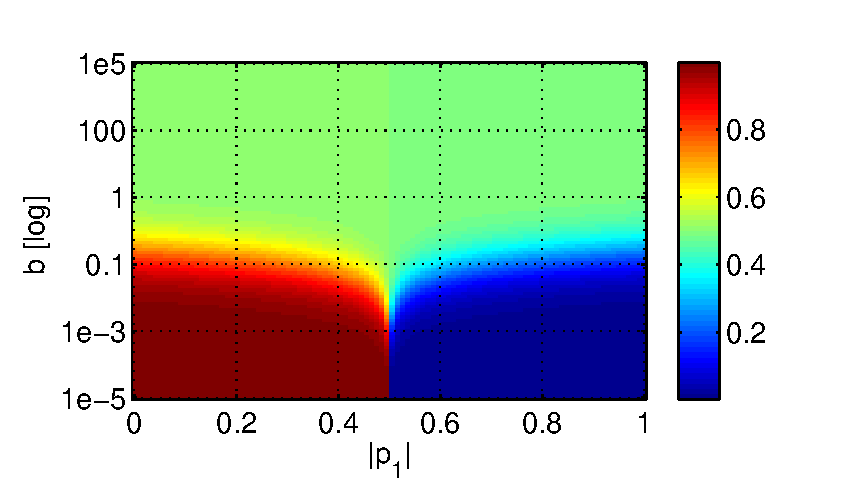
\includegraphics[width=0.80\textwidth]{figs/probability.eps}
\caption{Example of the distribution over 2 tasks.}
\label{fig:probability_example}
\end{center}
\end{figure}

As noted above we denote by $Z_{i,t}=1$ iff $i=J_t$.
The update of the algorithm is performed with the perceptron rule,
that is $\vwi{J_t,t} = \vwi{J_t,t-1}+M_{J_t,t} \, \yi{J_t,t}\,
\vxi{J_t,t}$ and $\vwi{i,t} = \vwi{i,t-1}$ for $i \neq J_t$. 
For simplicity of presentation we write the update for all of the tasks in one term  as, $\vwi{i,t} =
\vwi{i,t-1} + Z_{i,t}\, M_{i,t} \, \yi{i,t}\, \vxi{i,t}$. One can notice that although
this notation uses labels for all tasks,  %(via $M_{i,t}$)
onlythe label of the task $J_t$ is used in practice, as for other tasks $Z_{i,t}=0$.
We call this algorithm {\em SHAMPO} for SHared Annotator for Multiple PrOblems. 
The pseudo-code of this algorithm appears  in \algoref{alg:SHAMPO_FO}.

The following theorem states that the expected cumulative number of mistakes
that the algorithm makes, may not be higher than for an algorithm that
observes the labels of all inputs. 
\begin{theorem}
  If SHAMPO algorithm runs on $K$ tasks with $K$ parallel example pair
  sequences
  $(\vxi{i,1},y_{i,1}),\ldots,(\vxi{i,n},y_{i,n})\in\mathbb{R}^d\times\{-1,1\}$,
  $i=1,...,K$ with input parameter $b>0$, then for all $\gamma>0$, all
  $\vui{i}\in\mathbb{R}^d$ and all $n\ge1$, there exists $0<\delta\le K$, such that,
  
\begin{equation}\label{eq:bound_FO_SHAMPO}
\mathbb{E}\left[ \sum_{i=1}^{K}\sum_{t=1}^{n}{M_{i,t}} \right]
\le \frac{\delta}{\gamma}\brackets{\left(1+\frac{X^2}{2b} \right){\bar L}_{\gamma,n}
+\frac{\braces{2b+X^2}^2\tilde{U}^2}{8{\gamma}b}}~,
\end{equation}
 where $X=\max_{i,t}\Vert\vxiit\Vert$,
$\tilde{U}^2=\sum_{i=1}^{K}\normt{\vui{i}}$ and the expectation is over the
random choices of the algorithm.
\end{theorem} \label{thm:FO_theorem}

\begin{algorithm}[h]
\begin{algorithmic}
   \State \textbf{Parameters:}  $b\in\mathbb{R}>0$.
   \State \textbf{Initialize:} $\vwi{i,0}=\vzero$ for $i=1\comdots K$\\
   \For {$t=1,2,\ldots, n$} 
\begin{enumerate}
\nolineskips
\item Observe $K$ instance vectors, $\vxiit$, ($i=1 \comdots K$).
\item Compute margins $\hat{p}_{i,t}=\vwti{i,t-1} \vxiit$.
\item Predict $K$ labels, $\hyi{i,t}=\sign(\hat{p}_{i,t})$.
\item Draw task $J_t$  with the distribution:
\begin{align}
\pr{J_t=j} &=
\frac{\paren{b+\abs{\hat{p}_{j,t}}-\min_{m=1}^K\abs{\hat{p}_{m,t}}}^{-1}}{D_{t}}, \nonumber\\
D_t &=
\sum_i \paren{b+\abs{\hat{p}_{i,t}}-\min_{m=1}^K\abs{\hat{p}_{m,t}}}^{-1}. \nonumber
\end{align}
\item Query the true label ,$\yi{J_t,t}\in\{-1,1\}$.
\item Set the indicator $M_{J_t, t}=1$ iff $\yi{J_t,t} \neq \hyi{J_t,t}$.
\item Update with the perceptron rule:
\begin{align}
&\vwi{J_t,t} = \vwi{J_t,t-1}+M_{J_t,t} \, \yi{J_t,t}\, \vxi{J_t,t}\label{eq:update_rule} \\
&\vwi{i,t} ~~= \vwi{i,t-1}  \textrm{ for } i \neq J_t \nonumber
\end{align}
\end{enumerate}
   \EndFor  
   \State {\bf Output}: $\vwi{i,n}$ for $i=1 \comdots K$.
\end{algorithmic}
\caption{SHAMPO:\@ SHared Annotator for Multiple PrOblems.}\label{alg:SHAMPO_FO}
\end{algorithm}

\begin{proof}
Fix $n$ examples sequences, $(\vxi{i,1},y_{i,1}),\ldots,(\vxi{i,n},y_{i,n})$ for each one of the $K$ tasks. 
Let $t$ be certain trial and $i$ to be an update task on this trial, such that $M_{i,t}=1$. 
We can write,
\begin{align*}
\gamma-\lossp{\gamma,i,t}(\vu_i)&=\gamma-\paren{\gamma-y_{i,t}\vu_i^T\vxiit}_+\\
 ~&\le~  y_{i,t}\vu_i^{T}\vxiit \\
&= y_{i,t}\paren{\vu_i+\vwi{i,t-1}-\vwi{i,t-1}}^{T}\vxiit\\
&= y_{i,t}\vwi{i,t-1}^{T}\vxiit+\paren{\vu_i-\vwi{i,t-1}}^{T}y_{i,t}\vxiit\\
&= y_{i,t}\vwi{i,t-1}^{T}\vxiit+\paren{\vu_i-\vwi{i,t-1}}^{T}\paren{\vwi{i,t}-\vwi{i,t-1}}\\
&=  y_{i,t}\vwi{i,t-1}^{T}\vxiit+\frac{1}{2}{\normt{\vu_{i}-\vwi{i,t-1}}}
        -\frac{1}{2}{\normt{\vu_i-\vwiit}}+\frac{1}{2}{\normt{\vwi{i,t-1}-\vwiit}}\\
&=  y_{i,t}\hat{p}_{i,t}+\frac{1}{2}{\normt{\vu_{i}-\vwi{i,t-1}}}
        -\frac{1}{2}{\normt{\vu_i-\vwiit}}+\frac{1}{2}{\normt{\vwi{i,t-1}-\vwiit}}~.
\end{align*}

\noindent
The last inequality holds for all $\gamma>0$ and for all
$\vu_i\in\mathbb{R}^d$, so we can replace $\gamma$ and $\vu_i$ by their
scaling $\alpha\gamma$ and $\alpha \vu_i$ respectively, where $\alpha>0$
is a scaling parameter that will be determined shortly. Since the inequality is computed on an update task,
$y_{i,t}\hat{p}_{i,t}\le0$ holds , i.e. $y_{i,t}\hat{p}_{i,t}=-\abs{\hat{p}_{i,t}}$ , and we get

\begin{equation*}
\begin{split}
\alpha\gamma  +&\abs{\hat{p}_{i,t}} \le\\
&\alpha\lossp{\gamma,i,t}(\vu_i)+\frac{1}{2}{\normt{\alpha \vu_i-\vwi{i,t-1}}}-\frac{1}{2}{\normt{\alpha \vu_i-\vwiit}}+\frac{1}{2}{\normt{\vwi{i,t-1}-\vwiit}} .\end{split}
\end{equation*}

\noindent
Now, in order to generalize the inequality, we multiply it by the indicator $M_{i,t}Z_{i,t}$ , 
which means that the inequality holds for  trials and tasks where there is an update, as stated above.

\begin{equation*}
\begin{split}
M_{i,t}&Z_{i,t}{\paren{\alpha\gamma \!-\!\abs{\hat{p}_{i,t}}}} \!\le\! M_{i,t}Z_{i,t}\alpha \lossp{\gamma,i,t}(\vu_i)
+\\ &\frac{M_{i,t}Z_{i,t}}{2}\normt{\alpha \vu_i\!-\!\vwi{i,t\!-\!1}}\!-\!\frac{M_{i,t}Z_{i,t}}{2}\normt{\alpha \vu_i\!-\!\vwiit}\!+\!
\frac{M_{i,t}Z_{i,t}}{2}\normt{\vwi{i,t\!-\!1}\!-\!\vwiit}\!.
\end{split}
\end{equation*} 

 \noindent
Yet, in the other cases,  when no update is performed and  $M_{i,t}Z_{i,t}=0$,
the equality $\vwiit=\vwi{i,t-1}$ holds as well, so we can rid off the indicator for any one of the last three 
terms and we have

\begin{equation*}
\begin{split}
M_{i,t}Z_{i,t}{\paren{\alpha\gamma +\abs{\hat{p}_{i,t}}}} \le M_{i,t}&Z_{i,t}\alpha \lossp{\gamma,i,t}(\vu_i)+\\ 
\frac{1}{2}\normt{\alpha \vu_i-\vwi{i,t-1}}&-\frac{1}{2}\normt{\alpha \vu_i-\vwiit}+
\frac{M_{i,t}Z_{i,t}}{2}\normt{\vwi{i,t-1}-\vwiit}.
\end{split}
\end{equation*}

\noindent
Next, we sum the inequality above, over $t$,  recall the facts that
$\vwi{i,0}=0$ and $\normt{\vwi{i,t-1}-\vwiit}\le X^2$ for $X=\max_{i,t}\Vert\vxiit\Vert$ to get,

\begin{equation}
\begin{split}
\sum_{t=1}^{n}{M_{i,t}Z_{i,t}{\paren{\alpha\gamma+\abs{\hat{p}_{i,t}}-\frac{X^2}{2}}}}
\le\alpha\sum_{t=1}^{n}{ M_{i,t}Z_{i,t}
  \lossp{\gamma,i,t}(\vu_i)}&+\frac{\alpha^2}{2}\normt{\vu_i}.
\end{split}
\label{step_1_in_proof}
\end{equation}

\noindent
Substituting $\alpha=(2b+X^2)/2\gamma$ (where $b\in\mathbb{R},~~b>0$)
in ~\eqref{step_1_in_proof}, we get
\begin{equation*}
\begin{split}
\sum_{t=1}^{n}{M_{i,t}Z_{i,t}{\paren{b +\abs{\hat{p}_{i,t}}}}}
\le \frac{2b+X^2}{2\gamma}\sum_{t=1}^{n}{ M_{i,t}Z_{i,t}\lossp{\gamma,i,t}(\vu_i)}
+\frac{\left({2b+X^2}\right)^2}{8{\gamma}^2}\normt{\vu_i}.
\end{split}
\end{equation*} 

\noindent
Now, we subtract a non negative quantity $\sum_{t=1}^{n}M_{i,t}Z_{i,t}
{{\min_j{\abs{\hat{p}_{j,t}}}}}$ from the l.h.s. and get,
\begin{equation}
\begin{split}
\sum_{t=1}^{n}M_{i,t}Z_{i,t}{\paren{b +\abs{\hat{p}_{i,t}}-\min_j{\abs{\hat{p}_{j,t}}}}}&\le\\
\frac{2b+X^2}{2\gamma}\sum_{t=1}^{n}{ M_{i,t}Z_{i,t}}&\lossp{\gamma,i,t}(\vu_i)
+\frac{\left({2b+X^2}\right)^2}{8{\gamma}^2}\normt{\vu_i}.
\label{step_2_in_proof}
\end{split}
\end{equation}

\noindent
At this point we take  the expectation of all the terms.  Recall that the conditional expectation of $Z_{i,t}$ is 
$(b+|\hat{p}_{i,t}|-\min_j| \hat{p}_{j,t}|)^{-1}/D_{t}$
and that $M_{i,t}$ and $\hat{p}_{i,t}$ are measurable with respect to the $\sigma$-algebra that generated by $Z_1,\ldots,Z_{t-1}$. 
We start with the left term,
\begin{align*}
\begin{split}
&\mathbb{E}\brackets{\sum_{t=1}^{n}M_{i,t}Z_{i,t}{\paren{{b
        +\abs{\hat{p}_{i,t}}}-\min_{j}{\abs{ \hat{p}_{j,t}}}}}}= \\
        &\mathbb{E}\brackets{\mathbb{E}_{t-1}\brackets{{\sum_{t=1}^{n}{M_{i,t}Z_{i,t}{\left({b +\abs{\hat{p}_{i,t}}}-\min_{j}{\abs{\hat{p}_{j,t}}}\right)}}}}}= \\
&\mathbb{E}\brackets{{\sum_{t=1}^{n}M_{i,t}{\left({b +\left\vert{\hat{p}_{i,t}}\right\vert}-\min_{j}{\left\vert \hat{p}_{j,t} \right\vert}\right)}\mathbb{E}_{t-1}\brackets{ Z_{i,t}}}}=\\
&\mathbb{E}\brackets{\sum_{t=1}^{n}{\frac{M_{i,t}}{D_{t}}}}~.
\end{split}
\end{align*}

\noindent
Substituting the last term in the expectation of
\eqref{step_2_in_proof}, % we get,
\begin{equation}
\mathbb{E}\left[ \sum_{t=1}^{n}{\frac{M_{i,t}}{D_{t}}} \right]
\le \frac{2b+X^2}{2\gamma}{\bar
  L}_{\gamma,i,n}(u_i)+\frac{\left({2b+X^2}\right)^2}{8{\gamma}^2}{\left\Vert
    \vui{i} \right\Vert}^2~.
\label{step_3_in_proof}
\end{equation} 

\noindent
Since that the normalization factor is a sum of positive components,
hence $D_t$ is maximal when each of the components gets its maximal
value. This happens when $\left\vert \hat{p}_{m,t}
\right\vert=\left\vert \hat{p}_{j,t} \right\vert ~~  \forall
m,j \in\{1,\ldots K\}$. This allows us to bound the normalization factor as
follows,
\begin{equation*}
D_{t}=\sum_{m=1}^{K}{\left({b+\left\vert \hat{p}_{m,t}
      \right\vert-\min_{j}{\left\vert \hat{p}_{j,t}
        \right\vert}}\right)^{-1}} \le \sum_{m=1}^{K}{b^{-1}}=\frac{K}{b}~.
\end{equation*}


\noindent
Since $M_{i,t}>0 ~\forall{i,t}$, thus there exists $\delta_i\in\reals>0$ such that 
\begin{equation}
\label{eq:introducing_delta}
\mathbb{E}\brackets{\sum_{t=1}^{n}{\frac{M_{i,t}}{D_{t}}}} = 
\frac{b}{\delta_i}\mathbb{E}\brackets{\sum_{t=1}^{n}{M_{i,t}}}.
\end{equation}
and
\begin{equation}
\frac{b}{\delta_i} \geq \min\frac{1}{D_t}  = \frac{1}{\max D_t}  \geq 
\frac{b}{K}~.
\label{eq:FO_bound_on_D}
\end{equation}

\noindent
Which implies that $0<\delta_i\le K$.\\
Plugging ~\eqref{eq:introducing_delta} in ~\eqref{step_3_in_proof} we get,
\begin{equation*}
\frac{b}{\delta_i}\mathbb{E}\left[ \sum_{t=1}^{n}{M_{i,t}} \right]
\le \frac{2b+X^2}{2\gamma}{\bar L}_{\gamma,i,n}(\vui{i})+\frac{\left({2b+X^2}\right)^2}{8{\gamma}^2}{\left\Vert \vui{i} \right\Vert}^2.
\end{equation*}

\noindent
Summing up the last inequality over all $K$ tasks and setting $\delta
= \max_i \delta_i$ yields, 
\begin{equation}
\begin{split}
\frac{1}{\delta}\mathbb{E}\left[ \sum_{i=1}^{K}\sum_{t=1}^{n}{M_{i,t}} \right]
\le\frac{1}{\gamma}\left(1+\frac{X^2}{2b} \right){\bar L}_{\gamma,n}+
\frac{\left({2b+X^2}\right)^2}{8{\gamma}^2b}\sum_{i=1}^{K}{{\left\Vert \vui{i} 
\right\Vert}^2}~,
\end{split}
\label{eq:FO_final_eq_in_proof}
\end{equation}
which concludes the proof.
\QED
\end{proof}

\noindent
One can use the bound to tune the algorithm for an optimal value of
$b$. However, this may not be possible as unfortunately ${\bar L}_{\gamma,n}$ depends
implicitly on the value of $b$\ (Similar issue appears also 
after the discussion of Theorem~1 in a different context by~\cite{cesa2006worst}).

\noindent
Alternatively, we can take a
loose estimate of ${\bar L}_{\gamma,n}$, and replace it with
$L_{\gamma,n}$ (which is $\sim K$ times larger). The optimal value of
$b$ can be now calculated, 
\begin{displaymath}
b=\frac{X^2}{2}{\sqrt{1+\frac{4\gamma L_{\gamma,n}}{U^{2}X^2}}}.
\end{displaymath}
Substituting this value in the bound of ~\eqref{eq:bound_FO_SHAMPO} with
$L_{\gamma,n}$ leads to the following bound, 
\begin{equation*}
\mathbb{E}\brackets{\sum_{i=1}^{K}\sum_{t=1}^{n}{M_{i,t}}}
\le\frac{\delta}{\gamma}\brackets{L_{\gamma,n}+\frac{U^{2}X^2}{2\gamma}+\frac{U^{2}}{2\gamma}\sqrt{1+\frac{4\gamma L_{\gamma,n}}{U^{2}X^2}}}
\end{equation*}
which has the same dependency in the number of inputs $n$ as algorithm
that observes all of them.

We continue now with an analysis of an extension of our
algorithm that allows more than a single query per round. In this setting, the ability  
of the annotator to annotate data instances is less limited. Here, we
allow the algorithm to query $\kappa$ labels at a time ( $\kappa<K$), instead of one. On each
iteration $t$, the modified algorithm samples without repetitions,
$\kappa$ labels to be annotated, and perform the same update as of
\eqref{eq:update_rule}. Formally, on each round we have $\sum_i
Z_{i,t}=\kappa$ for $Z_{i,t}\in\{0,1\}$ where the first task-index to
be queried is
drawn according to ~\eqref{eq:prob}. The second task is drawn from the
same distribution, eliminating the first choice and adjusting the normalization factor, and so on. Once
$\kappa$ problems are drawn, the algorithm receives $\kappa$ labels for
the $\kappa$ corresponding inputs, and updates the $\kappa$ models
according to ~\eqref{eq:update_rule}.

\noindent
\begin{corollary}
  If SHAMPO algorithm gets feedback for $\kappa$ tasks on each round,
  instead of only a single problem, the expected cumulative weighted
  mistakes is bounded as follows
\begin{displaymath}
\mathbb{E}\left[ \sum_{i=1}^{K}\sum_{t=1}^{n}{M_{i,t}} \right] 
\le \frac{1}{C(\kappa,K)}\paren{\frac{1}{\gamma}\left(1+\frac{X^2}{2b} \right){\bar L}^\kappa_{\gamma,n}
+\kappa\frac{\left({2b+X^2}\right)^2}{8{\gamma}^2b}\tilde{U}^2}~,
\end{displaymath}
where $C(\kappa,K) = \sum_{j=K-\kappa+1}^{K}\frac{1}{j}$ , and
${\bar L}^\kappa_{\gamma,n}$ is the expected loss of $K$ models
$\{\vui{i}\}$ over the $\kappa$ instances that are annotated per round
$t$.
\end{corollary}

\noindent
\begin{proof}
We follow the proof of \thmref{thm:FO_theorem} until \eqref{eq:FO_final_eq_in_proof}, recall $\delta_i < K$. We
  repeat the process $\kappa$ times, and get the equivalent inequality
  for sampling $\kappa$ problems without repetitions,
\begin{equation}
\begin{split}
  \paren{\sum_{j=K-\kappa+1}^{K}\frac{1}{j}}\mathbb{E}\left[ \sum_{i=1}^{K}\sum_{t=1}^{n}{M_{i,t}} \right]
\le \frac{1}{\gamma}\left(1+\frac{X^2}{2b} \right){\bar L}^\kappa_{\gamma,n}
+\kappa\frac{\left({2b+X^2}\right)^2}{8{\gamma}^2b} U^2~,
\end{split}
\label{final_eq_k}
\end{equation}
where all expectations are now with respect to the sampling
repetitions, and specifically ${\bar L}^\kappa_{\gamma,n}$ is the
expected loss of a set of linear models $\{ \vui{i} \}$ where $\kappa$
problems are sampled rather than a single one.
\QED

% in \eqref{eq:bound_for_i} we saw a bound for the expectation of the sum of errors for the case of $K$ tasks. After we chose one task and got it's feedback, we want to choose another task to issue a query on in the same way. Now we have $K-1$ tasks and the bound
% \begin{equation}
% \sum_{t=1}^{n}\Exp{M_{i,t}\frac{b}{K-1}}
% \le \frac{2b+X^2}{2\gamma}{\bar L}_{\gamma,i,n}(\vui{i})+\frac{\left({2b+X^2}\right)^2}{8{\gamma}^2}{\left\Vert \vui{i} \right\Vert}^2
% \end{equation}
% when $i\ne J_t$. Now we can choose another task out of the $K-2$ tasks and so on. summing over all of the tasks we get the bound expectation of the weight errors over time and tasks
% \begin{equation}
% \Exp{\sum_{t=1}^{n}\brackets{\sum_{J=1}^{\kappa-1}M_{J,t}\frac{1}{K+1-J}+\sum_{i=\kappa }^{K}M_{i,t}\frac{1}{K+1-\kappa}}}
% \le \frac{2b+X^2}{2b\gamma}{\bar L}_{\gamma,n}+\frac{\left({2b+X^2}\right)^2}{8b{\gamma}^2}U.
% \end{equation}
 
\end{proof}

\noindent
It can be shown that this bound  is a generalized form of \thmref{thm:FO_theorem}. 
For $\kappa=1$ we get the bound of \thmref{thm:FO_theorem} (with $\delta = K$), while for
$\kappa=K$ we have $C(\kappa,K)>\ln(K+1)$, thus recovering the
bound of $K$ Perceptron trained in parallel, with a sightly ($1/\ln(K+1)$)
worse dependency in the number of tasks.

\section{Aggressive version}

So far we used the margin to build the distribution over the tasks,  but in the update stage,
we used the same regular perceptron update rule, that makes an update only when there is a prediction 
mistake. However, we already said that the margin can tells us about the uncertainty in the prediction, 
so it may be helpful to proceed with this approach in the update stage as well and make the sharp update 
threshold a little bit softer. 

In this  version of SHAMPO algorithm, the update is been preformed not only when there is a mistake, 
but also in the case of correct prediction with low margin, i.e. low certainty. We define this margin to be
$\lambda \in\reals>0$. In addition to the previous mistake indicator, $M_{i,t}$,  we introduce one more 
indicator,  $G_{i,t}$. We keep the notation of  $M_{i,t}=1$ when there is wrong prediction on the task $i$
in round $t$ and $M_{i,t}=0$ otherwise, and set $G_{i,t}=1$ when there is no prediction mistake on the task 
$i$ in round $t$, but the margin is lower than our threshold, i.e. $0<\abs{\hat{p}_{i,t}}<\lambda,$ therefore an
aggressive update takes place, and $G_{i,t}=0$  otherwise. 
An update is performed if either there is a mistake ($M_{J_i,t}=1$) or the margin is
low ($G_{J_i,t}=1$). Note that these events are mutually exclusive thus, for simplicity, we define the update
indicator which is  $U_{i,t}=M_{i,t}+G_{i,t}$. This indicator is  $U_{i,t}=1$ on update trials and  $U_{i,t}=0$
when no update has been made.

\begin{algorithm}[h]
\begin{algorithmic}
   \State \textbf{Parameters:}  $b, \lambda \in\mathbb{R}>0$.
   \State \textbf{Initialize:}  $\vwi{i,0}=\vzero$ for $i=1\comdots K$ \\
   \For {$t=1,2,\ldots, n$} 
\begin{enumerate}
\nolineskips
\item Observe $K$ instance vectors, $\vxiit$, ($i=1 \comdots K$).
\item Compute margins $\hat{p}_{i,t}=\vwti{i,t-1} \vxiit$.
\item Predict $K$ labels, $\hyi{i,t}=\sign(\hat{p}_{i,t})$.
\item Draw problem $J_t$  with the distribution:
\begin{align}
\pr{J_t=j} &=
\frac{\paren{b+\abs{\hat{p}_{j,t}}-\min_{m=1}^K\abs{\hat{p}_{m,t}}}^{-1}}{D_{t}}, ~\nonumber\\
D_t &=
\sum_i \paren{b+\abs{\hat{p}_{i,t}}-\min_{m=1}^K\abs{\hat{p}_{m,t}}}^{-1}. \nonumber
\end{align}
\item Query the true label ,$\yi{J_t,t}\in\{-1,1\}$.
\item Set the indicator $M_{J_t, t}=1$ iff $\yi{J_t,t} \neq \hyi{J_t,t}$.
\item Iff $M_{J_t, t}=0$ and $\abs{p_{J_t,t}}<\lambda$, set  the indicator $G_{J_t,t}=1$
\item For $U_{i,t}=M_{i,t}+G_{i,t}$ update with the perceptron rule:
\begin{align}
&\vwi{J_t,t} = \vwi{J_t,t-1}+U_{J_t,t} \, \yi{J_t,t}\, \vxi{J_t,t}  \nonumber\\
&\vwi{i,t} ~~= \vwi{i,t-1}  \textrm{ for } i \neq J_t \nonumber
\end{align}
\end{enumerate}
   \EndFor  
   \State {\bf Output}: $\vwi{i,n}$ for $i=1 \comdots K$.
\end{algorithmic}
\caption{SHAMPO aggressive perceptron.}
\label{alg:SHAMPO_FO_aggressive}
\end{algorithm}    


  


\begin{theorem}
  If Aggressive SHAMPO algorithm runs on $K$ problems with $K$ parallel example pair
  sequences
  $(\vxi{i,1},y_{i,1}),\ldots,(\vxi{i,n},y_{i,n})\in\mathbb{R}^d\times\{-1,1\}$,
  $i=1,...,K$ with input parameters $b>0$, and $0 \le \lambda \le b/2$ then for all $\gamma>0$, all
  $\vui{i}\in\mathbb{R}^d$ and all $n\ge1$, there exists $0<\delta\le K$, such that,
  
\begin{displaymath}
\begin{split}
\mathbb{E}\left[ \sum_{i=1}^{K}\sum_{t=1}^{n}{M_{i,t}} \right]
\le \frac{\delta}{\gamma}&\brackets{\left(1+\frac{X^2}{2b} \right){\bar L}_{\gamma,n}
+\frac{\left({2b+X^2}\right)^2\tilde{U}^2}{8{\gamma}b}}\\ 
+&\paren{2\frac{\lambda}{b}-1}\mathbb{E}\brackets{\sum_{i=1}^{K}\sum_{t=1}^{n}{G_{i,t}}}~,
\label{bound_aggressive_FO_SHAMPO}
\end{split}
\end{displaymath}
 where $X=\max_{i,t}\Vert\vxiit\Vert$,
$\tilde{U}^2=\sum_{i=1}^{K}\normt{\vui{i}}$ and the expectation is over the
random choices of the algorithm.
\end{theorem} \label{thm:FO_bound_aggressive}

\noindent
The theorem above, states that when the update is aggressive, the bound on the expected number of errors
can be tighter than the non aggressive algorithm because we have added a new term to the bound 
which can be negative.     

In order to achieve tighter bound on the expected cumulative mistakes than we had in the regular SHAMPO 
perceptron algorithm (\thmref{thm:FO_theorem}), we need to restrict the aggressive margin  $\lambda$ 
to be $\lambda\le b/2$ so the last term will be negative. Indeed, one can say that this bound shows that the best choice of $\lambda$ is 
$\lambda=0$, i.e. it seems that aggressive update is not a good idea. However, in such case, 
$G_{i,t}=0,~ \forall i,t$ which means that this would not be the best choice of $\lambda$. 
This discrimination actually shows  that there is a sweet point where $0<\lambda<b/2$ such that the 
bound will be the  tightest as this bound allows . 

\begin{proof}
We follow the proof of $\thmref{thm:FO_theorem}$ on an update trial, reminding that now the update 
indicator is  $U_{i,t}=1, $ until we get,  

\begin{align*}
\gamma-&\lossp{\gamma,i,t}(\vu_i)\le \\
&y_{i,t}\hat{p}_{i,t}+\frac{1}{2}{\normt{\vu_{i}-\vwi{i,t-1}}}
        -\frac{1}{2}{\normt{\vu_i-\vwiit}}+\frac{1}{2}{\normt{\vwi{i,t-1}-\vwiit}}~.
\end{align*}
Whereas in the non aggressive version proof we claimed that $y_{i,t}\hat{p}_{i,t}=-\abs{\hat{p}_{i,t}}$ in an 
update trial, here, it is not true when an aggressive update takes place since we update when the prediction 
is correct as well. For that reason, we  remain with the term $y_{i,t}\hat{p}_{i,t}$ as is for now and we will 
deal with it later. In addition, in this proof,  we change the update indicator from $M_{i,t}$ to $U_{i,t}$. 
Considering these two changes, we proceed the proof until $\eqref{step_2_in_proof}$. Now we have,

\begin{equation}
\begin{split}
\sum_{t=1}^{n}U_{i,t}Z_{i,t}{\paren{b -y_{i,t}\hat{p}_{i,t}-\min_j{\abs{\hat{p}_{j,t}}}}}&\le\\
\frac{2b+X^2}{2\gamma}\sum_{t=1}^{n}U_{i,t}Z_{i,t}&\lossp{\gamma,i,t}(\vu_i)+\frac{\left({2b+X^2}\right)^2}{8{\gamma}^2}\normt{\vu_i}.
\label{eq:step_3_in_proof_agressive}
\end{split}
\end{equation}
 Since the inequality is computed on an update task, there is a need to discriminate between   the two possible options: either 
$y_{i,t}\hat{p}_{i,t}\le0$ holds  when there is prediction mistake ($M_{i,t}=1$), i.e. $y_{i,t}\hat{p}_{i,t}=-\abs{\hat{p}_{i,t}}$  ,  or $0\le y_{i,t}\hat{p}_{i,t}\le\lambda$ holds  when the prediction is correct,  but an aggressive update occurs ($G_{i,t}=1$) and  in that case  $y_{i,t}\hat{p}_{i,t}=\abs{\hat{p}_{i,t}}$.

At this point we take  the expectation of all the terms as before taking into consideration the two cases.  Recall that the conditional expectation of $Z_{i,t}$ is
$(b+|\hat{p}_{i,t}|-\min_j| \hat{p}_{j,t}|)^{-1}/D_{t}$
and that $M_{i,t}$ and $G_{i,t}$ (therefor also $U_{i,t}$) and $\hat{p}_{i,t}$ are measurable with respect to the $\sigma$-algebra that generated by $Z_1,\ldots,Z_{t-1}$. 
We start with the left term,
\begin{align*}
\begin{split}
&\mathbb{E}\brackets{\sum_{t=1}^{n}U_{i,t}Z_{i,t}{\paren{b-y_{i,t}\hat{p}_{i,t}-\min_{j}{\abs{ \hat{p}_{j,t}}}}}}\\
&=\mathbb{E}\brackets{\mathbb{E}_{t-1}\brackets{{\sum_{t=1}^{n}{U_{i,t}Z_{i,t}{\left(b-y_{i,t}\hat{p}_{i,t}-\min_{j}{\abs{\hat{p}_{j,t}}}\right)}}}}} \\
&=\mathbb{E}\brackets{{\sum_{t=1}^{n}U_{i,t}{\left({b -y_{i,t}\hat{p}_{i,t}}-\min_{j}{\left\vert \hat{p}_{j,t} \right\vert}\right)}\mathbb{E}_{t-1}\brackets{ Z_{i,t}}}}\\
&=\mathbb{E}\brackets{\sum_{t=1}^{n}\frac{\paren{M_{i,t}+G_{i,t}}}{D_{t}}\frac{\paren{b -y_{i,t}\hat{p}_{i,t}-\min_{j}\abs{\hat{p}_{j,t}}}}{b+\abs{\hat{p}_{i,t}}-\min_{j}{\abs{\hat{p}_{j,t}}}}}\\
&=\mathbb{E}\brackets{\sum_{t=1}^{n}{\frac{1}{D_{t}}\paren{M_{i,t}+\frac{b-\abs{\hat{p}_{i,t}}-\min_{j}{\abs{\hat{p}_{j,t}} }}{b+\abs{\hat{p}_{i,t}}-\min_{j}{\abs{\hat{p}_{j,t}}}}G_{i,t} }}}~.
\end{split}
\end{align*}

\noindent
Substituting the last term in the expectation of
\eqref{eq:step_3_in_proof_agressive} we get,
\begin{equation}
\begin{split}
\mathbb{E}\left[ \sum_{t=1}^{n}{\frac{1}{D_{t}}}\paren{M_{i,t}+\frac{b-\abs{\hat{p}_{i,t}}-\min_{j}{\abs{\hat{p}_{j,t}} }}{b+\abs{\hat{p}_{i,t}}-\min_{j}{\abs{\hat{p}_{j,t}}}}G_{i,t} } \right]
&\le \\ \frac{2b+X^2}{2\gamma}{\bar
  L}_{\gamma,i,n}(u_i)+&\frac{\left({2b+X^2}\right)^2}{8{\gamma}^2}{\left\Vert
    \vui{i} \right\Vert}^2~.
\label{step_3_in_proof_aggressive}
\end{split}
\end{equation} 

\noindent
Now we bound the factor that is multiplied by $G_{i,t}$ using the fact that $G_{i,t}=1$ only when 
$\abs{\hat{p}_{i,t}}<\lambda$ ,
\begin{equation}
\label{eq:bound_on_agressive_multiplier}
\paren{1-2\frac{\lambda}{b}}=\frac{b-2\lambda}{b} \le\frac{b-\abs{\hat{p}_{i,t}}-\min_{j}{\abs{\hat{p}_{j,t}} }}{b+\abs{\hat{p}_{i,t}}-\min_{j}{\abs{\hat{p}_{j,t}}}}\le1.
\end{equation}

\noindent
We can use now \eqref{eq:bound_on_agressive_multiplier} to substitute the left hand 
side of \eqref{step_3_in_proof_aggressive} with the lower term

\begin{equation*}
\mathbb{E}\brackets{
  \sum_{t=1}^{n}{\frac{1}{D_{t}}}\paren{M_{i,t}+\paren{1-2\frac{\lambda}{b}}G_{i,t}}}.
\end{equation*}

\noindent
Since $b/2 \geq \lambda$ we have that
$M_{i,t}+\paren{1-2\frac{\lambda}{b}}G_{i,t}\geq 0$,  and as stated before in \eqref{eq:FO_bound_on_D}, 
there exists $\delta_i\in\reals,~ 0<\delta_i\le K$ such that, 
\begin{equation*}
\mathbb{E}\left[
  \sum_{t=1}^{n}{\frac{1}{D_{t}}}\paren{M_{i,t}+\paren{1-2\frac{\lambda}{b}}G_{i,t}
  } \right]=\frac{b}{\delta_i}\mathbb{E}\left[
  \sum_{t=1}^{n}\paren{M_{i,t}+\paren{1-2\frac{\lambda}{b}}G_{i,t}
  } \right] ~.
\end{equation*}

\noindent
Plugging this in ~\eqref{step_3_in_proof_aggressive} we get,
\begin{equation*}
\begin{split}
\frac{b}{\delta_i}\mathbb{E}\brackets{\sum_{t=1}^{n}{M_{i,t}}}
\le& \frac{2b+X^2}{2\gamma}{\bar L}_{\gamma,i,n}(\vui{i})\\
&+\frac{\left({2b+X^2}\right)^2}{8{\gamma}^2}{\left\Vert \vui{i} \right\Vert}^2+ 
     \frac{b}{\delta_i}\paren{2\frac{\lambda}{b}-1}\mathbb{E}\brackets{\sum_{t=1}^{n}{G_{i,t}}}.
\end{split}
\end{equation*}

\noindent
Summing up the last inequality over all $K$ tasks and setting $\delta
= \max_i \delta_i$ yields,
\begin{equation*}
\begin{split}
\frac{1}{\delta}\mathbb{E}\left[ \sum_{i=1}^{K}\sum_{t=1}^{n}{M_{i,t}} \right]
\le&\frac{1}{\gamma}\left(1+\frac{X^2}{2b} \right){\bar L}_{\gamma,n}\\
&+\frac{\left({2b+X^2}\right)^2}{8{\gamma}^2b}\sum_{i=1}^{K}{{\left\Vert \vui{i} \right\Vert}^2}+ \frac{1}{\delta}\paren{2\frac{\lambda}{b}-1}\mathbb{E}\brackets{\sum_{i=1}^{K}\sum_{t=1}^{n}{G_{i,t}}}
\end{split}
\end{equation*}
Which concludes the proof
\QED
\end{proof}

\section{prior distribution over tasks}

We saw before that $b$ is a tradeoff parameter between  exploitation and uniform  distribution over the 
tasks (exploration). It is possible that we have prior knowledge about the tasks, which tasks are harder than 
the others. In this case, we would like to add this prior knowledge to the distribution such that in the 
exploration will be done with  a prior distribution. This is especially important in the first steps of the 
algorithms when instead starting in pure uniform exploration (since we initialize our model vectors, $\vwi{i,0}=\vzero$)  
we can start with a reasonable prior distribution.
In order to do that we change the probability to be 

\begin{equation*}
\pr{J_t=j} =
\frac{1}{D_{t}}\frac{a_{j}}{\paren{b+\abs{\hat{p}_{j,t}}-\min_{m=1}^K\abs{\hat{p}_{m,t}}}} \end{equation*}
where $a_j>1~~\forall j\in\braces{1,\ldots,K}$ and  $D_t$ is the normalization factor. We can use this distribution with the SHAMPO perceptron algorithm, but we would like to analyse the bound of the SHAMPO aggressive perceptron algorithm because it's more global. 

\begin{theorem}
  If Aggressive SHAMPO algorithm with prior runs on $K$ problems with $K$ parallel example pair
  sequences
  $(\vxi{i,1},y_{i,1}),\ldots,(\vxi{i,n},y_{i,n})\in\mathbb{R}^d\times\{-1,1\}$,
  $i=1,...,K$ with input parameters $b>0$, and $\lambda>0$  and $a_i>1~\forall i\in\braces{1,\cdots,K}$ then for all $\gamma>0$, all
  $\vui{i}\in\mathbb{R}^d$ and all $n\ge1$,
  
\begin{displaymath}
\begin{split}
\mathbb{E}\left[ \sum_{i=1}^{K}\sum_{t=1}^{n}{M_{i,t}} \right]
\le\frac{\sum_{j=1}^Ka_{j}}{\gamma}\brackets{\left(1+\frac{X^2}{2b} \right){\bar L}_{\gamma,n}+
\frac{\left({2b+X^2}\right)^2\tilde{U}^2}{8{\gamma}b}}\\ 
+
\paren{2\frac{\lambda}{b}-1}\mathbb{E}\brackets{\sum_{i=1}^{K}\sum_{t=1}^{n}{a_{i}G_{i,t}}},
\label{bound_FO_SHAMPO_prior}
\end{split}
\end{displaymath}
 where $X=\max_{i,t}\Vert\vxiit\Vert$,
$\tilde{U}^2=\sum_{i=1}^{K}\normt{\vui{i}}$ and the expectation is over the
random choices of the algorithm.
\end{theorem} \label{thm:FO_bound_aggressive}
This bound brings an advantage and disadvantage. We can reduce the last term in the bound choosing the right weights for $a_i$, but then, we suffer the factor of $\sum_{j=1}^Ka_{j}$ in rest part of the bound. 
\\
\begin{proof}
We follow the proof of ~\sthmref{bound_aggressive_FO_SHAMPO} until ~\eqref{eq:step_3_in_proof_agressive}, 
than we take the expectation of this term. First, we take the expectation of the left hand side 
where now the conditional expectation of $Z_{i,t}$ changed to 
\[
\mathbb{E}\brackets{Z_{i,t}}=\frac{1}{D_{t}}\frac{a_{i}}{\paren{b+\abs{\hat{p}_{i,t}}-\min_{m=1}^K\abs{\hat{p}_{m,t}}}}.
\]
Doing that, the expectation becomes
\begin{align*}
\begin{split}
&\mathbb{E}\brackets{\sum_{t=1}^{n}U_{i,t}Z_{i,t}{\paren{b-y_{i,t}\hat{p}_{i,t}-\min_{j}{\abs{ \hat{p}_{j,t}}}}}} \\
        &=\mathbb{E}\brackets{\mathbb{E}_{t-1}\brackets{{\sum_{t=1}^{n}{U_{i,t}Z_{i,t}{\left(b-y_{i,t}\hat{p}_{i,t}-\min_{j}{\abs{\hat{p}_{j,t}}}\right)}}}}} \\
&=\mathbb{E}\brackets{\sum_{t=1}^{n}{\frac{a_{i}}{D_{t}}\paren{M_{i,t}+\frac{b-\abs{\hat{p}_{j,t}}-\min_{j}{\abs{\hat{p}_{j,t}} }}{b+\abs{\hat{p}_{j,t}}-\min_{j}{\abs{\hat{p}_{j,t}}}}G_{i,t} }}}~.
\end{split}
\end{align*}
Reminding that $a_{i} \ge 1 \forall i$, we can bound $M_{i,t} \le M_{i,t}a_{i}$ and get 
\begin{equation}
\begin{split}
\mathbb{E}\left[ \sum_{t=1}^{n}{\frac{1}{D_{t}}}\paren{M_{i,t}+\frac{b-\abs{\hat{p}_{j,t}}-\min_{j}{\abs{\hat{p}_{j,t}} }}{b+\abs{\hat{p}_{j,t}}-\min_{j}{\abs{\hat{p}_{j,t}}}}G_{i,t}a_{i} } \right]
&\le \\ \frac{2b+X^2}{2\gamma}{\bar
  L}_{\gamma,i,n}(u_i)+&\frac{\left({2b+X^2}\right)^2}{8{\gamma}^2}{\left\Vert
    \vui{i} \right\Vert}^2~.
\label{step_3_in_proof_prior}
\end{split}
\end{equation}
We use now the same bound as in ~\eqref{eq:bound_on_agressive_multiplier}
and plug it into the left side of the inequality,

\begin{multline*}
\mathbb{E}\brackets{\sum_{t=1}^{n}{\frac{1}{D_{t}}}\paren{M_{i,t}+\paren{1-2\frac{\lambda}{b}}G_{i,t}a_{i} }}
\le \\
\mathbb{E}\left[ \sum_{t=1}^{n}{\frac{1}{D_{t}}}\paren{M_{i,t}+\frac{b-\abs{\hat{p}_{j,t}}-\min_{j}{\abs{\hat{p}_{j,t}} }}{b+\abs{\hat{p}_{j,t}}-\min_{j}{\abs{\hat{p}_{j,t}}}}G_{i,t}a_{i} } \right].
\end{multline*}

Since $b/2 \geq \lambda$ we have that
$M_{i,t}+\paren{1-2\frac{\lambda}{b}}G_{i,t}a_{i}\geq 0$, thus there
exists $\delta_i$ such that, 

\begin{multline}
  \label{eq:bound_delta_prior}
\mathbb{E}\left[
  \sum_{t=1}^{n}{\frac{1}{D_{t}}}\paren{M_{i,t}+\paren{1-2\frac{\lambda}{b}}G_{i,t}a_{i}
  } \right]= \\
  \frac{b}{\delta_i}\mathbb{E}\left[
  \sum_{t=1}^{n}\paren{M_{i,t}+\paren{1-2\frac{\lambda}{b}}G_{i,t}a_{i}
  } \right] ~,
\end{multline}

and 
\[
\frac{b}{\delta_i} \geq \min\frac{1}{D_t}  = \frac{1}{\max D_t}  \geq \frac{b}{\sum_{j=1}^Ka_{j}}~,
\]
where the last inequality follows from,
\begin{equation}\label{eq:bound_D}
D_{t}=\sum_{j=1}^K\frac{a_{j}}{\paren{b+\abs{\hat{p}_{j,t}}-\min_{m=1}^K\abs{\hat{p}_{m,t}}}}\le \frac{\sum_{j=1}^Ka_{j}}{b}.
\end{equation}
The previous bound implies that $0<\delta_i\le\sum_{i=1}^Ka_{i  }$.

Combining ~\eqref{step_3_in_proof_prior} and ~\eqref{eq:bound_delta_prior}, 
\begin{multline}
\label{eq:bound_for_i}
\frac{b}{\delta_i}\mathbb{E}\left[ \sum_{t=1}^{n}{M_{i,t}} \right]
\le \frac{2b+X^2}{2\gamma}{\bar L}_{\gamma,i,n}(\vui{i}) 
\\+\frac{\left({2b+X^2}\right)^2}{8{\gamma}^2}{\left\Vert \vui{i} \right\Vert}^2 
+\frac{b}{\delta_i}\paren{2\frac{\lambda}{b}-1}a_{i}\mathbb{E}\brackets{\sum_{t=1}^{n}{G_{i,t}}}.
\end{multline}
Summing up the last inequality over all $K$ tasks and setting $\delta
= \max_i \delta_i$ yields,
\begin{equation}\label{eq:final_eq}
\begin{split}
\mathbb{E}\left[ \sum_{i=1}^{K}\sum_{t=1}^{n}{M_{i,t}} \right]
\le&\frac{\delta}{\gamma }\brackets{\left(1+\frac{X^2}{2b} \right){\bar L}_{\gamma,n}+
\frac{\left({2b+X^2}\right)^2}{8{\gamma}b}\sum_{i=1}^{K}{{\left\Vert \vui{i} \right\Vert}^2}}\\ 
&+
\paren{2\frac{\lambda}{b}-1}\mathbb{E}\brackets{\sum_{i=1}^{K}\sum_{t=1}^{n}{a_{i}G_{i,t}}}~,
\end{split}
\end{equation}
which concludes the proof.
\QED
\end{proof}

We see that when this  bound is a global bound for the last two algorithms. 
If we set $a_i=1, ~~\forall i\in\braces{1,\cdots,K}$ we get the same bound as  SHAMPO aggressive 
algorithm and if we update only when a prediction mistake occurs, it means that 
$G_{i,t}=0,~~\forall i\in\braces{a,\cdots,K},t>0$ and we get the bound of  the ordinary 
SHAMPO perceptron algorithm.

\section{Kernel-based SHAMPO}
SHAMPO algorithm can also be used with Kernels in order to get a non linear 
classifiers in case of non separated data set by transforming the feature vector $\vx$ to $\Phi(\vx)$.
Define the binary parameter $\alpha_{i,t} = Z_{i,t}M_{i,t}$, we can rewrite the weight vector $\vw_{i,t}$ in its 
dual form as a linar combination of the input vectors
\[
\vw_{i,t} = \vw_{i,t-1}+Z_{i,t}M_{i,t}y_{i,t}\vxiit =\sum_{s=1}^t{Z_{i,s}M_{i,s}y_{i,s}\vx_{i,s}} 
= \sum_{s=1}^t{\alpha_{i,s}y_{i,s}\vx_{i,s}}.
\]
Now wee can rid of the weight algorithm and only store $\alpha_{i,t}$ values. 
Doing that, we get a new representation of the margin
\[
\hat{p}_{i,t}=\vwti{i,t-1} \vxiit = 
\tran{\paren{\sum_{s=1}^t{\alpha_{i,s}y_{i,s}\vx_{i,s}}}}\vxiit = 
\sum_{s=1}^t{\alpha_{i,s}y_{i,s}\paren{\tran{\vx_{i,s}}\vxiit}}= \sum_{s=1}^t{\alpha_{i,s}y_{i,s}K(\vx_{i,s},\vxiit})}
\]
where $K(\vx,\vy)  = \tran{\Phi(\vx)}\Phi(\vy)$ is the kernel function that represents the inner product of 
a high dimension space. 
 



\section{SHAMPO perceptron with Adaptive $b$ parameter}

As it has been proved in the analysis and will be shown in experiments, the parameter $b$ can tune 
the distribution over the tasks between exploration and exploitation, yet, there is still a need to supply 
the algorithm with this input parameter. So far, all of the tasks sheared the same parameter $b$ which
was determined at the beginning of the algorithm and remained constant during the whole process. 
For this reason, once the initial parameters were supplied, the margin was the only factor that had a varying
influence on the distribution. Now, we would like to suggest another algorithm that allow us to
dominate the distribution using the number of updates for each task. 
We assume as in Cesa-Bianchi et al  ~\cite{cesa2006worst} that the algorithm makes more mistakes on harder task than easier one, so a natural choice 
at any time, can be one that set higher probability to the tasks that made more prediction mistakes up to 
the same time. 

The adaptive algorithm is similar to the one in \figref{sec:alg} with three variation in order to comply with this
intuition. Here we introduce two more variables per task. First, the scalar 
$N_{i,n} = \sum_{t=1}^n{Z_{i,t}M_{i,t}}$ that holds the number of updates that has been done for the 
$i^{th}$ task  up to time $n$.
For simplicity of analysis we will write it in it's recursive way $N_{i,t}=N_{i,t-1}+1$.
The second variable is $X_{i,t}$ which is holds at the end of each cycle,  
the maximal norm of the input vectors that were involved in the updates.  The algorithm still have a parameter $\beta$ to be 
determined, however, it has less influence on the distribution than the parameter $b$ in  \figref{sec:alg}.
Using those three new parameter we introduce the adaptive version of $b$
\[
b_{i,t-1}=\beta X_{i,t} \sqrt{1+N_{i,t-1}}
\]
 The adaptive version of the  SHAMPO perceptron algorithm is  described in  \figref{alg:SHAMPO_adaptive}. 

\begin{algorithm}[h]
\begin{algorithmic}
   \State \textbf{Parameters:}  $\beta\in\mathbb{R}>0$.
   \State \textbf{Initialize:} $\vwi{i,0}=\vzero$ for $i=1\comdots K$\\
   \For {$t=1,2, ..., n$} 
   \begin{enumerate}
\nolineskips
\item Observe $K$ instance vectors, $\vxiit$, ($i=1 \comdots K$).
\item Compute margins $\hat{p}_{i,t}=\vwti{i,t-1} \vxiit$.
\item Predict $K$ labels, $\hyi{i,t}=\sign(\hat{p}_{i,t})$.
\item Set $X_{i,t}=\max\paren{X_{i,t-1},\Vert\vxiit\Vert}$
\item Draw task $J_t$  with the distribution:
\begin{align}
\pr{J_t=j} &=
\frac{1}{D_t}\frac{b_{i,t}}{b_{i,t}+\abs{\hat{p}_{j,t}}-\min_{m=1}^K\abs{\hat{p}_{m,t}}},\nonumber\\
D_t &=
\sum_i \frac{b_{i,t}}{b_{i,t}+\abs{\hat{p}_{j,t}}-\min_{m=1}^K\abs{\hat{p}_{m,t}}}.\nonumber
\end{align}
Where $b_{i,t} = \beta X_{i,t}^2\sqrt{1+N_{i,t}}$.
\item Query the true label ,$\yi{J_t,t}\in\{-1,1\}$.
\item Set the indicator $M_{J_t, t}=1$ iff $\yi{J_t,t} \neq \hyi{J_t,t}$.
\item Update with the perceptron rule:
\begin{align}
&\vwi{J_t,t} = \vwi{J_t,t-1}+M_{J_t,t} \, \yi{J_t,t}\, \vxi{J_t,t} \nonumber\\
&\vwi{i,t} ~~= \vwi{i,t-1}  \textrm{ for } i \neq J_t \nonumber\\
&N_{J_t,t} = N_{J_t,t} +M_{J_t,t} \nonumber
\end{align}
\end{enumerate}   \EndFor  
   \State {\bf Output}: $\vwi{i,n}$ for $i=1 \comdots K$.
\end{algorithmic}
\caption{Adaptive SHAMPO algorithm \label{alg:SHAMPO_adaptive}}
\end{algorithm}

\begin{theorem}
  If adaptive SHAMPO algorithm runs on $K$ tasks with $K$ parallel example pair
  sequences
  $(\vxi{i,1},y_{i,1}),...(\vxi{i,n},y_{i,n})\in\mathbb{R}^d\times\{-1,1\}$,
  $i=1,...,K$ with input parameter $b>0$, then for all $\gamma>0$, all
  $\vui{i}\in\mathbb{R}^d$ and all $n\ge1$, there exists $0<\delta\le K$, such that,
  
\begin{displaymath}
\mathbb{E}\brackets{ \sum_{i=1}^{K}\sum_{t=1}^{n}{M_{i,t}}}
\le \delta\brackets{\frac{\delta B^2}{2}+\frac{1}{\gamma}{\bar L}_{\gamma,n}+\frac{KR}{2\beta}
+ B\sqrt{\frac{\delta B^2}{4}+\frac{1}{\gamma}{\bar L}_{\gamma,n}+\frac{KR}{2\beta}}}
\end{displaymath}
 where $R = \max_i{\paren{\Vert u_i\Vert X_i}/{\gamma}}$, $B=\paren{R+\frac{2+3R}{2\beta}}$ and the expectation is over the
random choices of the algorithm.
\end{theorem} \label{thm:adaptive_bound}

 
The proof here is more  extended version of the proof in \thmref{thm:bound} . 
We will start here from ~\eqref{step_2_in_proof}. here, we will replace the constant scaling parameter, 
formerly $\alpha$, with a time varying factor $c_{i,t-1}/\gamma$, where $c_{i,t}\ge0$  is defined as following 

\begin{equation*}
c_{i,t-1}=\half\paren{\max{\braces{X_{i,t-1},\abs{\abs{\vxiit}}}}}+b_{i,t-1}.
\end{equation*}
Plugging the new scaling factor into the 
given inequality we get 
\begin{equation*}
\begin{split}
M_{i,t}Z_{i,t}{\paren{c_{i,t-1} +\abs{\hat{p}_{i,t}}}} \le M_{i,t}&Z_{i,t}\frac{c_{i,t-1}}{\gamma} \lossp{\gamma,i,t}(\vu_i)+\\ 
\frac{1}{2}\normt{\frac{c_{i,t-1}}{\gamma} \vu_i-\vwi{i,t-1}}&-\frac{1}{2}\normt{\frac{c_{i,t-1}}{\gamma} \vu_i-\vwiit}+
\frac{M_{i,t}Z_{i,t}}{2}\normt{\vwi{i,t-1}-\vwiit}.
\end{split}
\end{equation*}
From the update rule of the  algorithm we can bound $\normt{\vwi{i,t-1}-\vwiit}\le \normt{\vxiit}$. 
This inequality holds for any time step, and particular for an update iteration. 
Using this bound and dividing the inequality by  $b_{t-1}$ yields
\begin{equation}
\begin{split}
M_{i,t}Z_{i,t}&{\paren{\frac{c_{i,t-1} +\abs{\hat{p}_{i,t}}-\normt{\vxiit}/2}{b_{i,t-1}}}} \le M_{i,t}Z_{i,t}\frac{c_{i,t-1}}{b_{i,t-1}}\frac{\lossp{\gamma,i,t}(\vu_i)}{\gamma} \\ 
&+\frac{1}{2b_{i,t-1
}}\paren{\normt{\frac{c_{i,t-1}}{\gamma} \vu_i-\vwi{i,t-1}}-\normt{\frac{c_{i,t-1}}{\gamma} \vu_i-\vwiit}}.
\label{eq:adaptive_b_first_step}
\end{split}
\end{equation}
Now, we decompose the last term of the inequality to two  differences,
\begin{equation*}
\begin{split}
\frac{1}{2b_{i,t-1}}
\paren{\normt{\frac{c_{i,t-1}}{\gamma} \vu_i-\vwi{i,t-1}}-\normt{\frac{c_{i,t-1}}{\gamma} \vu_i-\vwiit}}= \\
\frac{1}{2b_{i,t-1}}\normt{\frac{c_{i,t-1}}{\gamma} \vu_i-\vwi{i,t-1}}-\frac{1}{2b_{i,t}}\normt{\frac{c_{i,t}}{\gamma} \vu_i-\vwi{i,t}}+\\
\frac{1}{2b_{i,t}}\normt{\frac{c_{i,t}}{\gamma} \vu_i-\vwi{i,t}}-\frac{1}{2b_{i,t-1}}\normt{\frac{c_{i,t-1}}{\gamma} \vu_i-\vwiit}.
\end{split}
\end{equation*}
At this point  expand the last two terms and  set   

and we get
\begin{equation*}
\begin{split}
\frac{1}{2b_{i,t}}\normt{\frac{c_{i,t}}{\gamma} \vu_i-\vwi{i,t}}&-\frac{1}{2b_{i,t-1}}\normt{\frac{c_{i,t-1}}{\gamma} \vu_i-\vwiit}\\
=&\frac{\normt{\vu_i}}{2\gamma^2}\paren{\frac{c_{i,t}^2}{b_{i,t}}-\frac{c_{i,t-1}^2}{b_{i,t-1}}}+
\frac{\vu_i^T\vwiit}{\gamma}\paren{\frac{c_{i,t-1}}{b_{i,t-1}}-\frac{c_{i,t}}{b_{i,t}}}\\
&+\frac{\normt{\vwiit}}{2}\paren{\frac{1}{b_{i,t}}-\frac{1}{b_{i,t-1}}}
\end{split}
\end{equation*}
We know that by definition, $b_{i,t}$ is non decreasing over time such that the last term is always negative 
and can be waved. In addition,  the definition of $c_{i,t}$  leads to 
\begin{equation*}
\frac{c_{i,t}}{b_{i,t}}=\frac{1}{2\beta\sqrt{1+N_{i,t}}}+1
\end{equation*}
which, combining with the fact that $N_{i,t}$ is nondecreasing over time as well, we get the inequality 
\begin{equation*}
\frac{c_{i,t}}{b_{i,t}}\le\frac{c_{i,t-1}}{b_{i,t-1}}
\end{equation*}
Combining these facts and using $Cauchy-Schwarz$ the inequality becomes,

\begin{equation}
\begin{split}
\frac{1}{2b_{i,t}}\normt{\frac{c_{i,t}}{\gamma} \vu_i-\vwi{i,t}}&-\frac{1}{2b_{i,t-1}}\normt{\frac{c_{i,t-1}}{\gamma} \vu_i-\vwiit}\\
\le&\frac{\normt{\vu_i}}{2\gamma^2}\paren{\frac{c_{i,t}^2}{b_{i,t}}-\frac{c_{i,t-1}^2}{b_{i,t-1}}}+
\frac{\Vert\vu_i\Vert~\Vert\vwiit\Vert}{\gamma}\paren{\frac{c_{i,t-1}}{b_{i,t-1}}-\frac{c_{i,t}}{b_{i,t}}}.
\end{split}
\label{eq:difference_of_norm_ineq}
\end{equation}
Here, recall that on an update trial $y_{i,t}\vw_{i,t-1}^{T}\vxiit\le0$ we define $X_i=\max_t{\Vert\vxiit\Vert}$ 
and use again the update rule and bound the weight vector norm with the number of updates , 
\begin{equation*}
\begin{split}
\normt{\vwiit}&=\normt{\vw_{i,t-1}+M_{i,t}Z_{i,t}y_{i,t}\vxiit}\\
&=\normt{\vw_{i,t-1}}+ 2M_{i,t}Z_{i,t}y_{i,t}\vw_{i,t-1}^{T}\vxiit+M_{i,t}Z_{i,t}\normt{\vxiit}\\
&\le\normt{\vw_{i,t-1}}+M_{i,t}Z_{i,t}\normt{\vxiit}\\
&\le\normt{\vw_{i,t-1}}+M_{i,t}Z_{i,t}X_i^2
\end{split}
\end{equation*}
Applying this inequality recursively, combined with the initial value $\vw_{i,0}=0$ leads us to
\begin{equation}
\Vert\vwiit\Vert\le X_i\sqrt{N_{i,t}}
\label{eq:bound_on_w}
\end{equation}
which holds for any $i$ and $t$. Combining the last inequality into  ~\eqref{eq:difference_of_norm_ineq} we get
\begin{equation}
\begin{split}
\frac{1}{2b_{i,t}}\normt{\frac{c_{i,t}}{\gamma} \vu_i-\vwi{i,t}}-\frac{1}{2b_{i,t-1}}\normt{\frac{c_{i,t-1}}{\gamma} \vu_i-\vwiit}\le\\
\frac{\normt{\vu_i}}{2\gamma^2}\paren{\frac{c_{i,t}^2}{b_{i,t}}-\frac{c_{i,t-1}^2}{b_{i,t-1}}}+
\frac{\Vert\vu_i\Vert~ X_i\sqrt{ N_{i,t}}}{\gamma}\paren{\frac{c_{i,t-1}}{b_{i,t-1}}-\frac{c_{i,t}}{b_{i,t}}}.
\label{eq:difference_of_norm_ineq_2}
\end{split}
\end{equation}
We will write now, a simpler bound on the last term. First we note that on $t$ that $M_{i,t}Z_{i,t}=1$, i.e. in the case of update, $N_{i,t}=N_{i,t-1}+1$. Using the bound $\sqrt{1+x}-\sqrt{x}\le\frac{1}{2\sqrt{x}}$, yields 
\begin{equation*}
\begin{split}
\sqrt{N_{i,t}}\paren{\frac{c_{t-1}}{b_{t-1}}-\frac{c_t}{b_t}}&=\frac{\sqrt{N_{i,t}}}{2\beta}\paren{\frac{1}{\sqrt{1+N_{i,t-1}}}-\frac{1}{\sqrt{1+N_{i,t}}}}\\
&=\frac{\sqrt{N_{i,t}}}{2\beta}\paren{\frac{1}{\sqrt{N_{i,t}}}-\frac{1}{\sqrt{1+N_{i,t}}}}\\
&=\frac{1}{2\beta}\frac{\sqrt{1+N_{i,t}}-\sqrt{N_{i,t}}}{\sqrt{1+N_{i,t}}}\\
&\le\frac{1}{4\beta}\frac{1}{\sqrt{N_{i,t}}\sqrt{1+N_{i,t}}}\\
&\le\frac{1}{4\beta}\frac{1}{N_{i,t}}.
\end{split}
\end{equation*} 
If $M_{i,t}Z_{i,t}=0$ , the left hand side becomes $0$ because in such case, $c_{i,t}=c_{i,t-1}$ and $b_{i,t}=b_{i,t-1}$, which means that this bound holds for all $i$ and $t$ and we can write it as  
\begin{equation*}
\begin{split}
\sqrt{N_{i,t}}\paren{\frac{c_{t-1}}{b_{t-1}}-\frac{c_t}{b_t}}
&\le\frac{M_{i,t}Z_{i,t}}{4\beta}\frac{1}{N_{i,t}}.
\end{split}
\end{equation*}
Plugging the  last bound and ~\eqref{eq:difference_of_norm_ineq_2} into ~\eqref{eq:adaptive_b_first_step} gives us the next inequality that holds for any $i,t,\gamma>0,$ and $u_i\in\reals^d$,
\begin{equation*}
\begin{split}
M_{i,t}Z_{i,t}&{\paren{\frac{c_{i,t-1} +\abs{\hat{p}_{i,t}}-\normt{\vxiit}/2}{b_{i,t-1}}}} \le M_{i,t}Z_{i,t}\frac{c_{i,t-1}}{b_{i,t-1}}\frac{\lossp{\gamma,i,t}(\vu_i)}{\gamma}\\
&+\frac{1}{2b_{i,t-1}}\normt{\frac{c_{i,t-1}}{\gamma} \vu_i-\vwi{i,t-1}}-\frac{1}{2b_{i,t}}\normt{\frac{c_{i,t}}{\gamma} \vu_i-\vwi{i,t}}\\
&+\frac{\normt{\vu_i}}{2\gamma^2}\paren{\frac{c_{i,t}^2}{b_{i,t}}-\frac{c_{i,t-1}^2}{b_{i,t-1}}}+
\frac{\Vert\vu_i\Vert~ X_i}{\gamma}\frac{M_{i,t}Z_{i,t}}{4\beta}\frac{1}{N_{i,t}}.
\end{split}
\end{equation*}
Recall the definition of $c_{i,t}$, we can write $c_{i,t-1}-\normt{\vxiit}/2\ge b_{i,t-1}$ and the ineqality gets the form
\begin{equation*}
\begin{split}
M_{i,t}Z_{i,t}&{\paren{\frac{b_{i,t-1} +\abs{\hat{p}_{i,t}}}{b_{i,t-1}}}} \le M_{i,t}Z_{i,t}\frac{c_{i,t-1}}{b_{i,t-1}}\frac{\lossp{\gamma,i,t}(\vu_i)}{\gamma}\\
&+\frac{1}{2b_{i,t-1}}\normt{\frac{c_{i,t-1}}{\gamma} \vu_i-\vwi{i,t-1}}-\frac{1}{2b_{i,t}}\normt{\frac{c_{i,t}}{\gamma} \vu_i-\vwi{i,t}}\\
&+\frac{\normt{\vu_i}}{2\gamma^2}\paren{\frac{c_{i,t}^2}{b_{i,t}}-\frac{c_{i,t-1}^2}{b_{i,t-1}}}+
\frac{\Vert\vu_i\Vert~ X_i}{\gamma}\frac{M_{i,t}Z_{i,t}}{4\beta}\frac{1}{N_{i,t}}.
\end{split}
\end{equation*}
Summing  both sides over $t=1,\cdots,n$, and taking into consideration the initialization,   $w_0=0$ we obtain,
\begin{equation}
\begin{split}
\sum_{t=1}^{n}M_{i,t}Z_{i,t}&{\paren{\frac{b_{i,t-1} +\abs{\hat{p}_{i,t}}}{b_{i,t-1}}}} \le \frac{1}{\gamma}\sum_{t=1}^{n}{M_{i,t}Z_{i,t}\frac{c_{i,t-1}}{b_{i,t-1}}\lossp{\gamma,i,t}(\vu_i)}\\
&+\frac{\normt{\vu_i}}{2\gamma^2}\frac{c_{i,n}^2}{b_{i,n}}-\frac{1}{2b_{i,n}}\normt{\frac{c_{i,n}}{\gamma} \vu_i-\vwi{i,n}}
+\frac{\Vert\vu_i\Vert~ X_i}{4\beta\gamma}\sum_{t=1}^{n}{\frac{M_{i,t}Z_{i,t}}{N_{i,t}}}.
\label{eq:first_sum}
\end{split}
\end{equation}
Now, we will bound the terms in the right hand side. The first term can be bounded as following,
\begin{equation*}
\begin{split}
\frac{1}{\gamma}\frac{c_{i,t-1}}{b_{i,t-1}}\lossp{\gamma,i,t}(\vu_i)&=\frac{1}{\gamma}\paren{\frac{1}{2\beta\sqrt{1+N_{i,t-1}}}+1}\lossp{\gamma,i,t}(\vu_i)\\
&\le \frac{1}{2\gamma\beta\sqrt{1+N_{i,t-1}}}\paren{\gamma+\Vert u_i\Vert X_i}+\frac{\lossp{\gamma,i,t}(\vu_i)}{\gamma}\\
&=\frac{1}{2\beta\sqrt{1+N_{i,t-1}}}\paren{1+\frac{\Vert u_i\Vert X_i}{\gamma}}+\frac{\lossp{\gamma,i,t}(\vu_i)}{\gamma}
\end{split}
\end{equation*}
Here, we used  the fact that $\lossp{\gamma,i,t}(\vu_i)\le \gamma+\Vert u_i\Vert X_i$.
Now we proceed  with  the two middle terms of ~\eqref{eq:first_sum} and get the bound
\begin{equation*}
\begin{split}
\frac{\normt{\vu_i}}{2\gamma^2}\frac{c_{i,n}^2}{b_{i,n}}-\frac{1}{2b_{i,n}}\normt{\frac{c_{i,n}}{\gamma} \vu_i-\vwi{i,n}}
&=\frac{c_{i,n}u_i^T\vwi{i,n}}{b_{i,n}\gamma}-\frac{\normt{\vw_{i,n}}}{2b_{i,n}}\\
&\le \frac{c_{i,n}u_i^T\vwi{i,n}}{b_{i,n}\gamma}\\
&\le\frac{c_{i,n}}{b_{i,n}}\frac{{\Vert u_i\Vert}~{\Vert\vwi{i,n}\Vert}}{\gamma}\\
&\le\paren{\frac{1}{2\beta\sqrt{1+N_{i,n}}}+1}\frac{{\Vert u_i\Vert}X_i\sqrt{N_{i,n}}}{\gamma},
\end{split}
\end{equation*}
where we used ~\eqref{eq:bound_on_w} in the last step.
Putting all together in ~\eqref{eq:first_sum}  gives us
\begin{equation*}
\begin{split}
\sum_{t=1}^{n}M_{i,t}Z_{i,t}&{\paren{\frac{b_{i,t-1} +\abs{\hat{p}_{i,t}}}{b_{i,t-1}}}}\\
\le &\frac{1}{2\beta}\paren{1+\frac{\Vert u_i\Vert X_i}{\gamma}}\sum_{t=1}^{n}{\frac{M_{i,t}Z_{i,t}}{\sqrt{1+N_{i,t-1}}}}
+\frac{1}{\gamma}\sum_{t=1}^{n}{M_{i,t}Z_{i,t}}\lossp{\gamma,i,t}(\vu_i)\\
+&\paren{\frac{1}{2\beta\sqrt{1+N_{i,n}}}+1}\frac{{\Vert u_i\Vert}X_i\sqrt{N_{i,n}}}{\gamma}
+\frac{\Vert\vu_i\Vert~ X_i}{4\beta\gamma}\sum_{t=1}^{n}{\frac{M_{i,t}Z_{i,t}}{N_{i,t}}}.
\end{split}
\end{equation*} 
The first and the last sums in the right hand side can get more elegant form. Recall $M_{i,t}Z_{i,t}=1$ implies $N_{i,t}=N_{i,t-1}+1$ , we can write  
\begin{equation*}
\begin{split}
\sum_{t=1}^{n}{\frac{M_{i,t}Z_{i,t}}{\sqrt{1+N_{i,t-1}}}}
=\sum_{t=1}^{n}{\frac{M_{i,t}Z_{i,t}}{\sqrt{N_{i,t}}}}
=\sum_{r=1}^{N_{i,n}}{\frac{1}{\sqrt{r}}} 
\le 2\sqrt{N_{i,n}}.
\end{split}
\end{equation*}
Now, we apply the same bound on the second sum, but with more loose bound, \begin{equation*}
\begin{split}
\sum_{t=1}^{n}{\frac{M_{i,t}Z_{i,t}}{N_{i,t}}}
\le\sum_{t=1}^{n}{\frac{M_{i,t}Z_{i,t}}{\sqrt{N_{i,t}}}} 
\le 2\sqrt{N_{i,n}}. 
\end{split}
\end{equation*}
Defining $R_i=\paren{\Vert u_i\Vert X_i}/{\gamma}$, and combining the last three bounds together we get
\begin{equation*}
\begin{split}
\sum_{t=1}^{n}M_{i,t}Z_{i,t}&{\paren{\frac{b_{i,t-1} +\abs{\hat{p}_{i,t}}}{b_{i,t-1}}}}\\
\le &\frac{1}{\gamma}\sum_{t=1}^{n}{M_{i,t}Z_{i,t}}\lossp{\gamma,i,t}(\vu_i)
+\frac{1}{\beta}\paren{1+\frac{3R_{i}}{2}}\sqrt{N_{i,n}}
\\
+&\frac{R_i}{2\beta}+R_{i}\sqrt{N_{i,n}}.
\end{split}
\end{equation*}
Now, we subtract non negative term from the left side, sum the inequality over all tasks and take 
the expectation.
\begin{equation*}
\begin{split}  
\mathbb{E}&\brackets{\sum_{i=1}^K\sum_{t=1}^{n}M_{i,t}Z_{i,t}{\paren{\frac{b_{i,t-1} +\abs{\hat{p}_{i,t}}-\min_j\abs{\hat{p}_{j,t}}}{b_{i,t-1}}}}}\\
\le &\frac{1}{\gamma}\mathbb{E}\brackets{\sum_{i=1}^K\sum_{t=1}^{n}{M_{i,t}Z_{i,t}}\lossp{\gamma,i,t}(\vu_i)}
+\mathbb{E}\brackets{\sum_{i=1}^K\paren{R_{i}+\frac{2+3R_{i}}{2\beta}}\sqrt{N_{i,n}}}\\
&+\mathbb{E}\brackets{\sum_{i=1}^{K}\frac{R_i}{2\beta}}.
\end{split}
\end{equation*}
First we look at the left hand side of the inequality.
\[
\sum_{i=1}^{K}\mathbb{E}&\brackets{\sum_{t=1}^{n}M_{i,t}Z_{i,t}{\paren{\frac{b_{i,t-1} +\abs{\hat{p}_{i,t}}-\min_j\abs{\hat{p}_{j,t}}}{b_{i,t-1}}}}}
= \sum_{i=1}^{K}\mathbb{E}\brackets{\sum_{t=1}^{n}\frac{M_{i,t}}{D_t}}
\]
The bound of $D_t$ now is 
\[
D_t = \sum_{i=1}^K{\frac{b_{i,t-1}}{b_{i,t-1} +\abs{\hat{p}_{i,t}}-\min_j\abs{\hat{p}_{j,t}}}}  
\le K
\]
Since $M_{i,t} > 0 \forall i,t$, thus there exists $\delta_i\in\reals >0$  such that
\[
\sum_{i=1}^{K}\mathbb{E}\brackets{\sum_{t=1}^{n}\frac{M_{i,t}}{D_t}} 
= \sum_{i=1}^{K}\frac{1}{\delta_i}\mathbb{E}\brackets{\sum_{t=1}^{n}M_{i,t}}  
\le\frac{1}{\delta}\mathbb{E}\brackets{\sum_{i=1}^{K}\sum_{t=1}^{n}M_{i,t}}  
\]
When $\delta = max_i{\delta_i}$.
Next we handle the middle term of the rhs.
\[
\begin{split}
\mathbb{E}&\brackets{\sum_{i=1}^K\paren{R_{i}+\frac{2+3R_{i}}{2\beta}}\sqrt{N_{i,n}}}
\le \mathbb{E}\brackets{\sum_{i=1}^K\paren{R+\frac{2+3R}{2\beta}}\sqrt{N_{i,n}}} \\
&=\paren{R+\frac{2+3R}{2\beta}}\mathbb{E}\brackets{\sum_{i=1}^K\sqrt{N_{i,n}}},
\end{split}
\]
Where $R=\max_i\paren{\Vert u_i\Vert X_i}/{\gamma}$.
Now, considering that $N_{i,n}$ is non-negative and and exploiting the concavity 
of the square root function we can continue as following
\[
\begin{split}
\mathbb{E}\brackets{\sum_{i=1}^K\sqrt{N_{i,n}}} 
&\le \mathbb{E}\brackets{\sqrt{K\sum_{i=1}^KN_{i,n}}}
=\sqrt{K}\mathbb{E}\brackets{\sqrt{\sum_{i=1}^KN_{i,n}}}\\
&\le \sqrt{K}\sqrt{\mathbb{E}\brackets{\sum_{i=1}^KN_{i,n}}}.
\end{split}
\]
Here we used the bound for sum of squares, $\sum_{i=1}^K\sqrt{a_i} \le \sqrt{K\sum_{i=1}^K a_i}$ 
for $a_i\in \reals, a_i\ge0$ combining with Jensen inequality. Moreover, we can 
continue, recall that by definition, $N_{i,n} = \sum_{t=1}^n{Z_{i,t}M_{i,t}}$ and $Z_{i,t}M_{i,t} \le M_{i,t}$ 
such that 
\[
\sqrt{K}\sqrt{\mathbb{E}\brackets{\sum_{i=1}^KN_{i,n}}} 
\le \sqrt{K}\sqrt{\mathbb{E}\brackets{\sum_{i=1}^K\sum_{t=1}^nM_{i,t}}}.
\]
Plugging the result in the inequality, we get
\begin{equation*}
\begin{split}
\frac{1}{\delta}\mathbb{E}&\brackets{\sum_{i=1}^{K}\sum_{t=1}^{n}M_{i,t}}\\
\le &\frac{1}{\gamma}\mathbb{E}\brackets{\sum_{i=1}^{K}\sum_{t=1}^{n}{M_{i,t}Z_{i,t}}\lossp{\gamma,i,t}(\vu_i)}
+\mathbb{E}\brackets{\sum_{i=1}^{K}\paren{R_{i}+\frac{2+3R_{i}}{2\beta}}\sqrt{N_{i,n}}}
+\mathbb{E}\brackets{\sum_{i=1}^{K}\frac{R_i}{2\beta}}\\
\le & \frac{1}{\gamma}{\bar L}_{\gamma,n}+\paren{R+\frac{2+3R}{2\beta}}\sqrt{K}\sqrt{\mathbb{E}\brackets{\sum_{i=1}^K\sum_{t=1}^nM_{i,t}}}
+\frac{KR}{2\beta}
\end{split}
\end{equation*}
which is quadratic inequality in  $\sqrt{\mathbb{E}\brackets{ \sum_{i=1}^{K}\sum_{t=1}^{n}{M_{i,t}} }$. 
Solving this equation gives us the bound for  the cumulative mistakes
\[
\mathbb{E}\brackets{ \sum_{i=1}^{K}\sum_{t=1}^{n}{M_{i,t}}}
\le \delta\brackets{\frac{\delta B^2}{2}+\frac{1}{\gamma}{\bar L}_{\gamma,n}+\frac{KR}{2\beta}
+ B\sqrt{\frac{\delta B^2}{4}+\frac{1}{\gamma}{\bar L}_{\gamma,n}+\frac{KR}{2\beta}}}
\]
\QED
